

\documentclass[english,11pt]{beamer}

\DeclareMathOperator{\Cov}{Cov}
\DeclareMathOperator{\Var}{Var}
\DeclareMathOperator{\E}{\mathbb{E}}
\DeclareMathOperator{\Proba}{\mathbb{P}}

\newcommand{\Covb}[2]{\ensuremath{\Cov\!\left[#1,#2\right]}}
\newcommand{\Eb}[1]{\ensuremath{\E\!\left[#1\right]}}
\newcommand{\Pb}[1]{\ensuremath{\Proba\!\left[#1\right]}}
\newcommand{\Varb}[1]{\ensuremath{\Var\!\left[#1\right]}}

% norm
\newcommand{\norm}[1]{\| #1 \|}

\newcommand{\indep}{\rotatebox[origin=c]{90}{$\models$}}





\usepackage{mathptmx,amsmath,amssymb,graphicx,bibentry,bbm,babel,ragged2e}

\makeatletter

\newcommand{\noun}[1]{\textsc{#1}}
\newcommand{\jitem}[1]{\item \begin{justify} #1 \end{justify} \vfill{}}
\newcommand{\sframe}[2]{\frame{\frametitle{#1} #2}}

\newenvironment{centercolumns}{\begin{columns}[c]}{\end{columns}}
%\newenvironment{jitem}{\begin{justify}\begin{itemize}}{\end{itemize}\end{justify}}

\usetheme{Warsaw}
\setbeamertemplate{footline}[text line]{}
\setbeamertemplate{headline}{}
\setbeamercolor{structure}{fg=purple!50!blue, bg=purple!50!blue}

\setbeamersize{text margin left=15pt,text margin right=15pt}

\setbeamercovered{transparent}


\@ifundefined{showcaptionsetup}{}{%
 \PassOptionsToPackage{caption=false}{subfig}}
\usepackage{subfig}

\usepackage[utf8]{inputenc}
\usepackage[T1]{fontenc}

\usepackage{multirow}

\usepackage{mdframed}


%\AtBeginSection[]
%{
%  \begin{frame}
%  \frametitle{}
%  \tableofcontents[currentsection]
%  \end{frame}
%}

\makeatother

\begin{document}



\title{Quantifying co-evolution of socio-economic activities with geo-historical data}

\author{J.~Raimbault$^{1,2,3,4, \ast}$\\
$\ast$\texttt{juste.raimbault@ign.fr}
}


\institute{$^{1}$LASTIG, Univ Gustave Eiffel, IGN-ENSG\\
$^{2}$CASA, UCL\\
$^{3}$UPS CNRS 3611 ISC-PIF\\
$^{4}$UMR CNRS 8504 G{\'e}ographie-cit{\'e}s
}


\date{\textit{3e journ{\'e}e du s{\'e}minaire SoDUCo-BnF}\\
23/05/2023
}




\frame{\maketitle}


\section{Introduction}

\sframe{Urban systems and geo-historical data}{


$\rightarrow$ Contemporary intra-urban dynamics are better and better characterised through the emergence of urban data and urban analytics \cite{kandt2021smart}; more difficult with past dynamics.

\bigskip

$\rightarrow$ Interdisciplinary approaches to the modeling of settlement systems transitions: qualitative or very sparse data, stylised models (Transmondyn project) \cite{sanders2018peupler}

\bigskip

$\rightarrow$ Stylised models for systems of cities on long time scales \cite{pumain2017urban}

\bigskip

$\rightarrow$ Difficulty to build geo-historical data: geocoding \cite{cura2018historical}, vectorisation \cite{el2022urban}

}


\sframe{Quantification of intra-urban co-evolutionary dynamics}{


$\rightarrow$ Multi-dimensionality of urban systems is one aspect of their complexity, strongly present in the co-evolution of economic activities locations.

\medskip

$\rightarrow$ Understanding past processes better inform urban theories and models for future sustainable planning.


\bigskip

\textbf{Research objective of this contribution (partly WP3): }

\medskip

\textit{Use geo-historical data to quantify the co-evolution of economic activities in Paris during the 19th century; methodological aspects on the issues linked to the exploitation of such data.}

}




\section{Data}

\sframe{Data extraction}{

% This contribution builds on data produced by the Soduco research project [9] to investigate co-evolutionary dynamics in the location of economic activities. More precisely, we focus on the case of Paris in the middle of the 19th cen- tury. Using public domain scans for main economic activ- ity repertoires (“Didot-Bottin”), an other work package of the project focused on building geo-referenced data contain- ing activities of various professionals, using Optical Char- acter Recognition techniques. 

% -> example of Didot?

%[9] Social dynamics in urban context. Open tools, models and data - Paris and its suburbs, 1789-1950. https://soduco.github.io/.



\begin{columns}
	\begin{column}{0.6\textwidth}
		\centering
		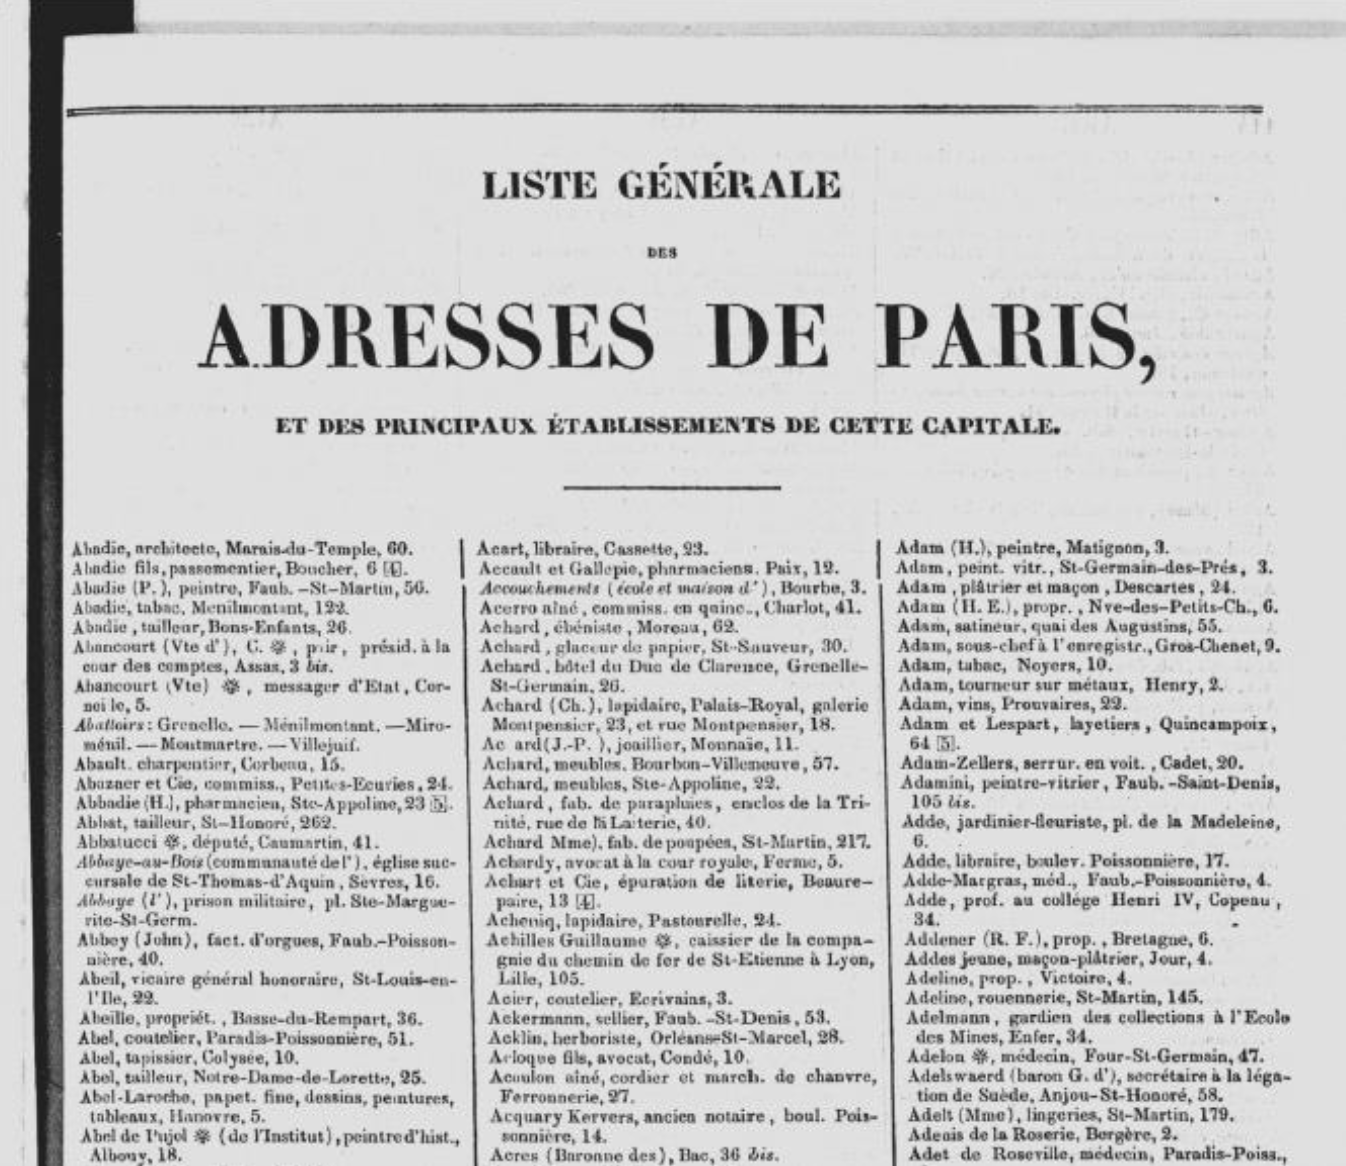
\includegraphics[width=\linewidth]{figures/didot.png}
	\end{column}
	\begin{column}{0.4\textwidth}
	
		\footnotesize
	
		\textit{Several commercial economic activities repertoires, archived and digitalised: cf previous seminars.}
		
		\bigskip
		
		\textit{Processing by other WPs of the SoDUCo project: }
		\begin{itemize}
			\item Document segmentation, OCR
			\item Named Entity Recognition to extract names, adresses, activities
			\item Historical geocoding
		\end{itemize}
		
		\bigskip
		
		$\rightarrow$ Work on \textit{Didot-Bottin}, covering most of 19th century (to avoid multi-source bias for now)
	\end{column}
\end{columns}




}


\sframe{Data pre-processing}{

% We work on a sample of this data currently available, spanning 4 years between 1841 and 1844.

% Starting from an initial dataset of 415,976 entries, we keep the ones with correct geographical coordinates (33%), and apply natural language processing (stemming and stop-word removal) to raw strings describing activities. From there, we focus on the stems with more than 100 occurences (578 stems), and code manually a broad category of economic activity for each (obtaining the coarse grain classification within: food, craftsmanship, art and literature, health, law and governance, service, teaching). We end at this stage with 36,072 entries with identified coordinates and broad ac- tivity. Source code and results are openly available on the git repository of this work at https://github.com/ JusteRaimbault/HistoricalData.

% New stats


$\rightarrow$ Data covering 1857-1908: 4,218,048 entries, 80.32\% with coordinates and a defined activity.

\bigskip

$\rightarrow$ Natural Language Processing: stop-words removal and stemming to descriptions of activities.

\bigskip

$\rightarrow$ Stems with more than 100 occurrences (996) coded for broad activities (food, craftsmanship, art and literature, health, law and governance, service, teaching)

\bigskip

$\rightarrow$ 1,990,222 entries with coordinates and classified activities




}


% includes "Methods"
\section{Results}


%\sframe{}{%
% plot: broad activities per year
%
%
%}


\sframe{Location of activities}{


\begin{center}
\hspace{-1cm}
	\includegraphics[width=0.49\textwidth, trim={0 0 4.5cm 0}]{figures/density-1857.png}\hspace{0.1cm}
	\includegraphics[width=0.49\textwidth, trim={0 0 4.5cm 0}]{figures/density-1908.png}
\end{center}


}


\sframe{Location of activities}{

% maps - to be redone !
% stored processed data? see other ordi tonight

\begin{center}
\hspace{-1cm}
	%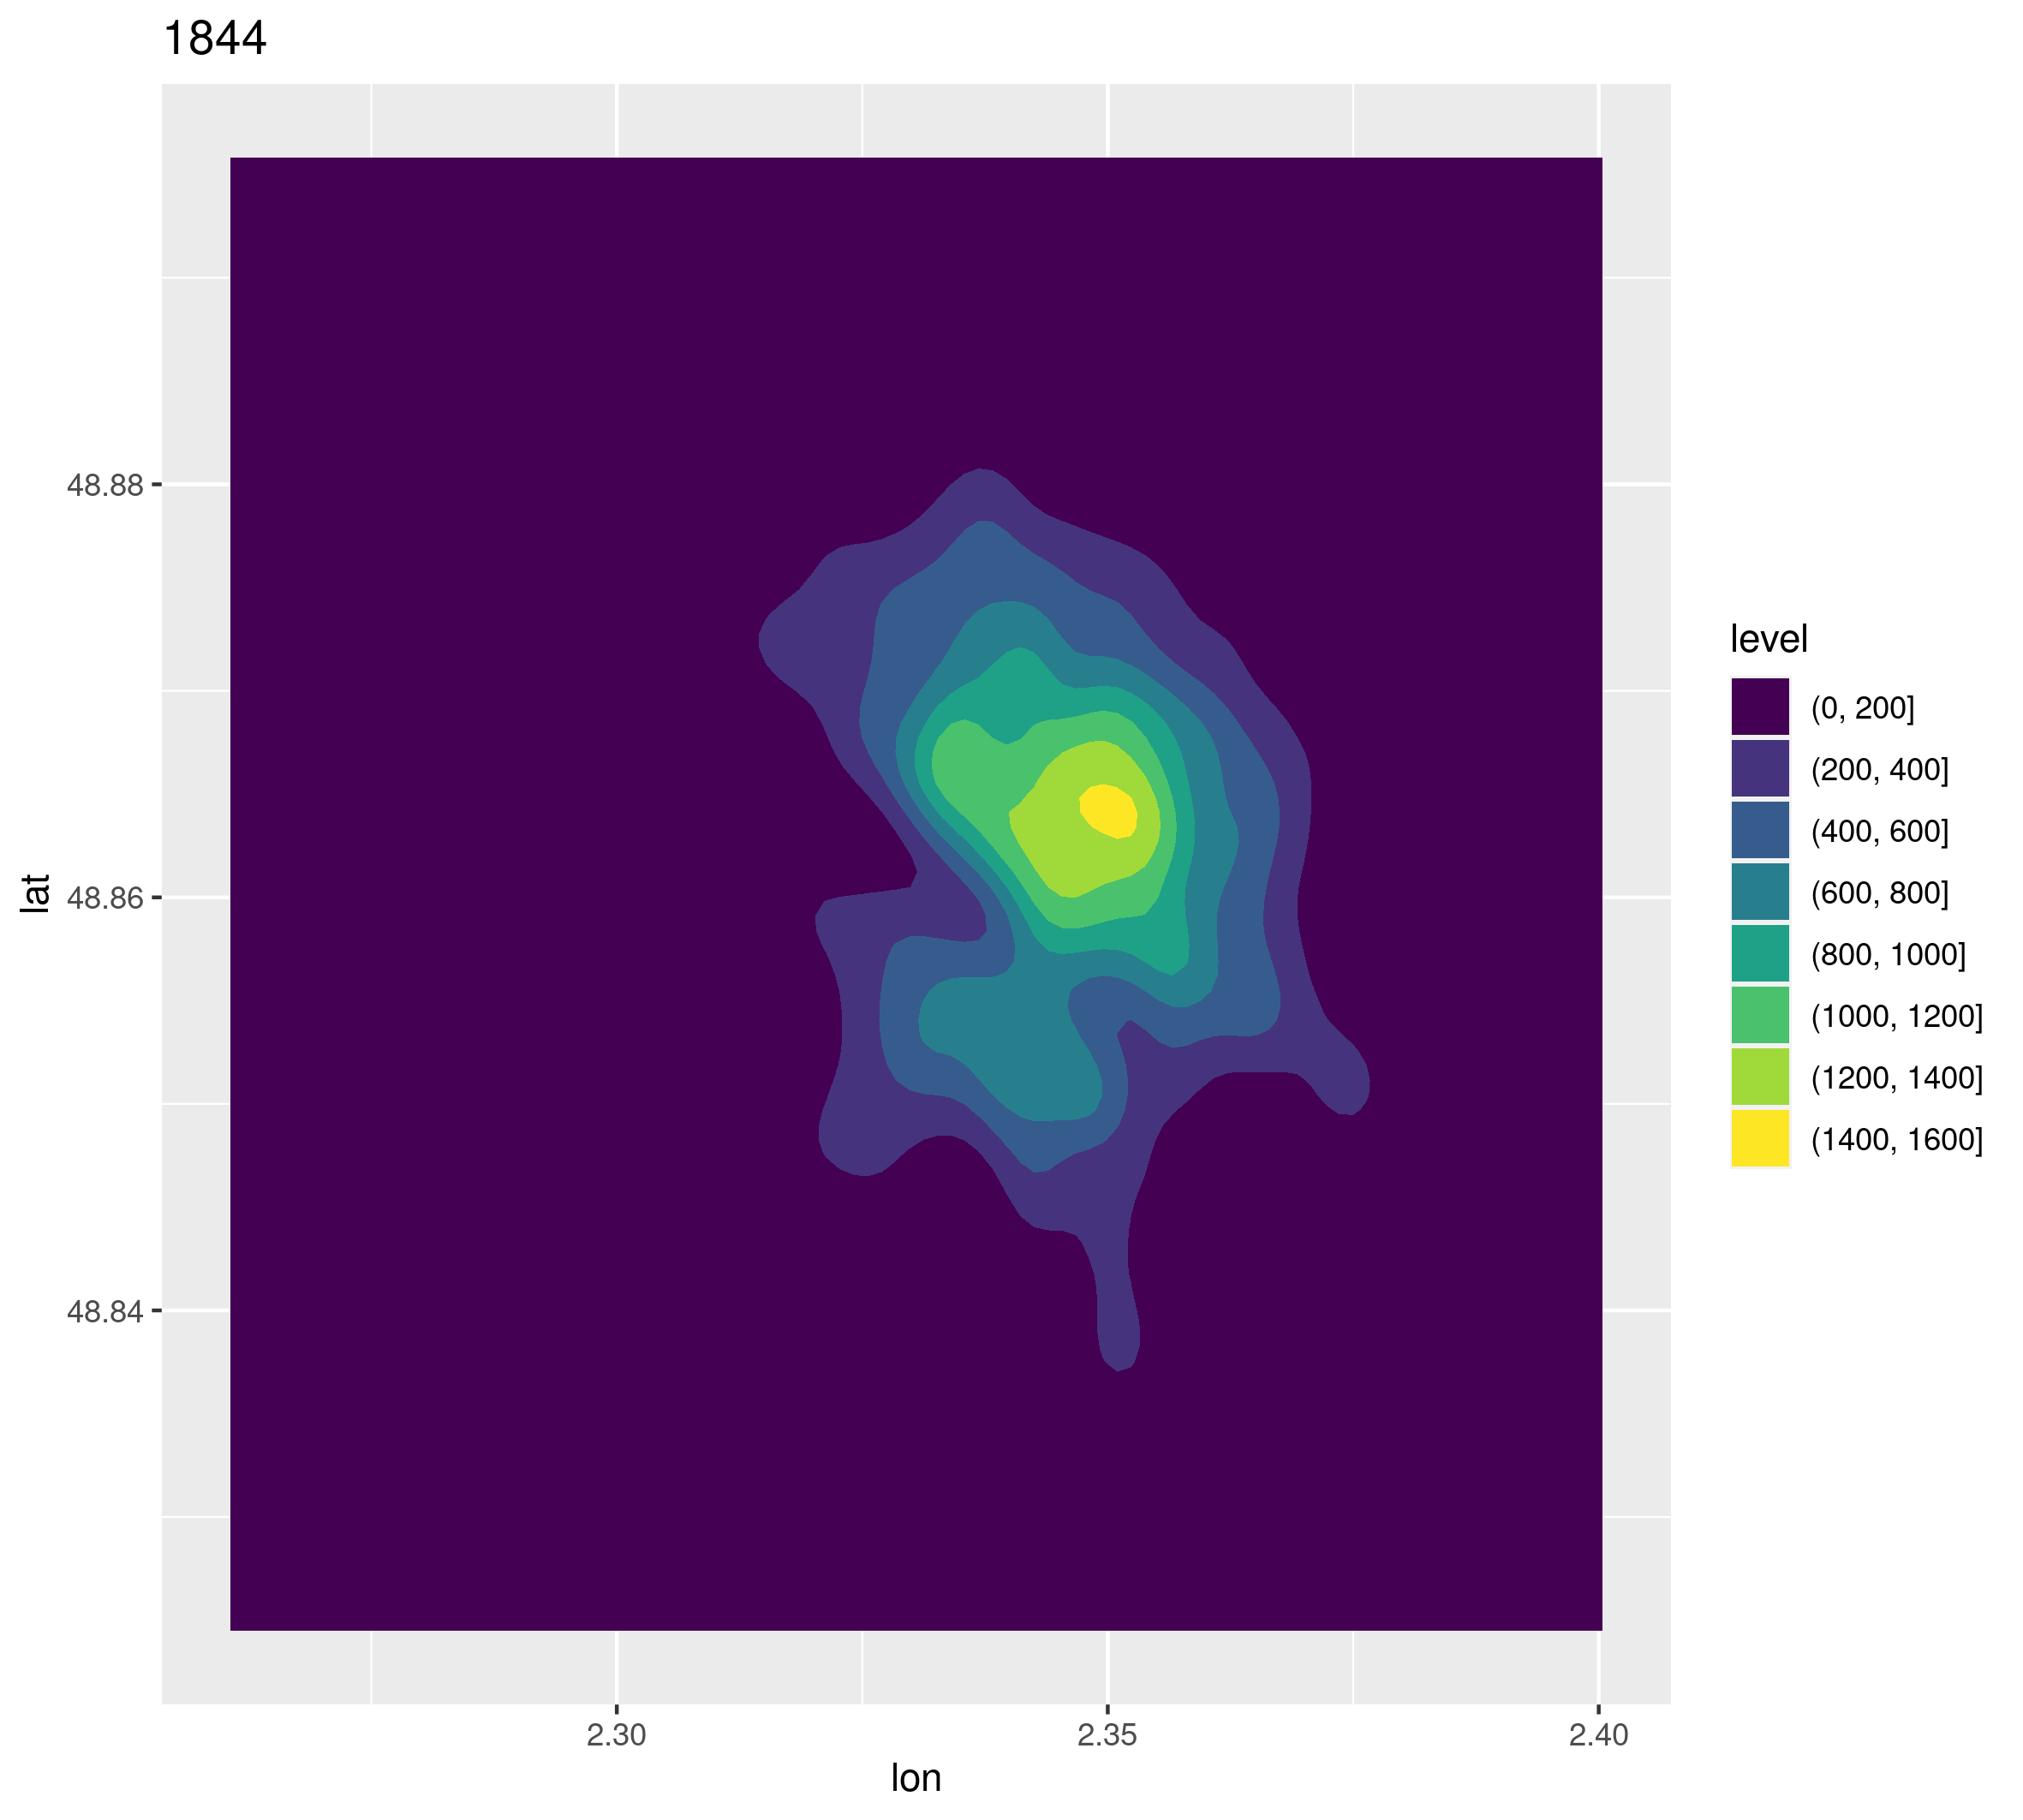
\includegraphics[width=0.49\textwidth, trim={0 0 4.5cm 0}]{figures/density-1844-craftsmanship.png}\hspace{0.1cm}
	%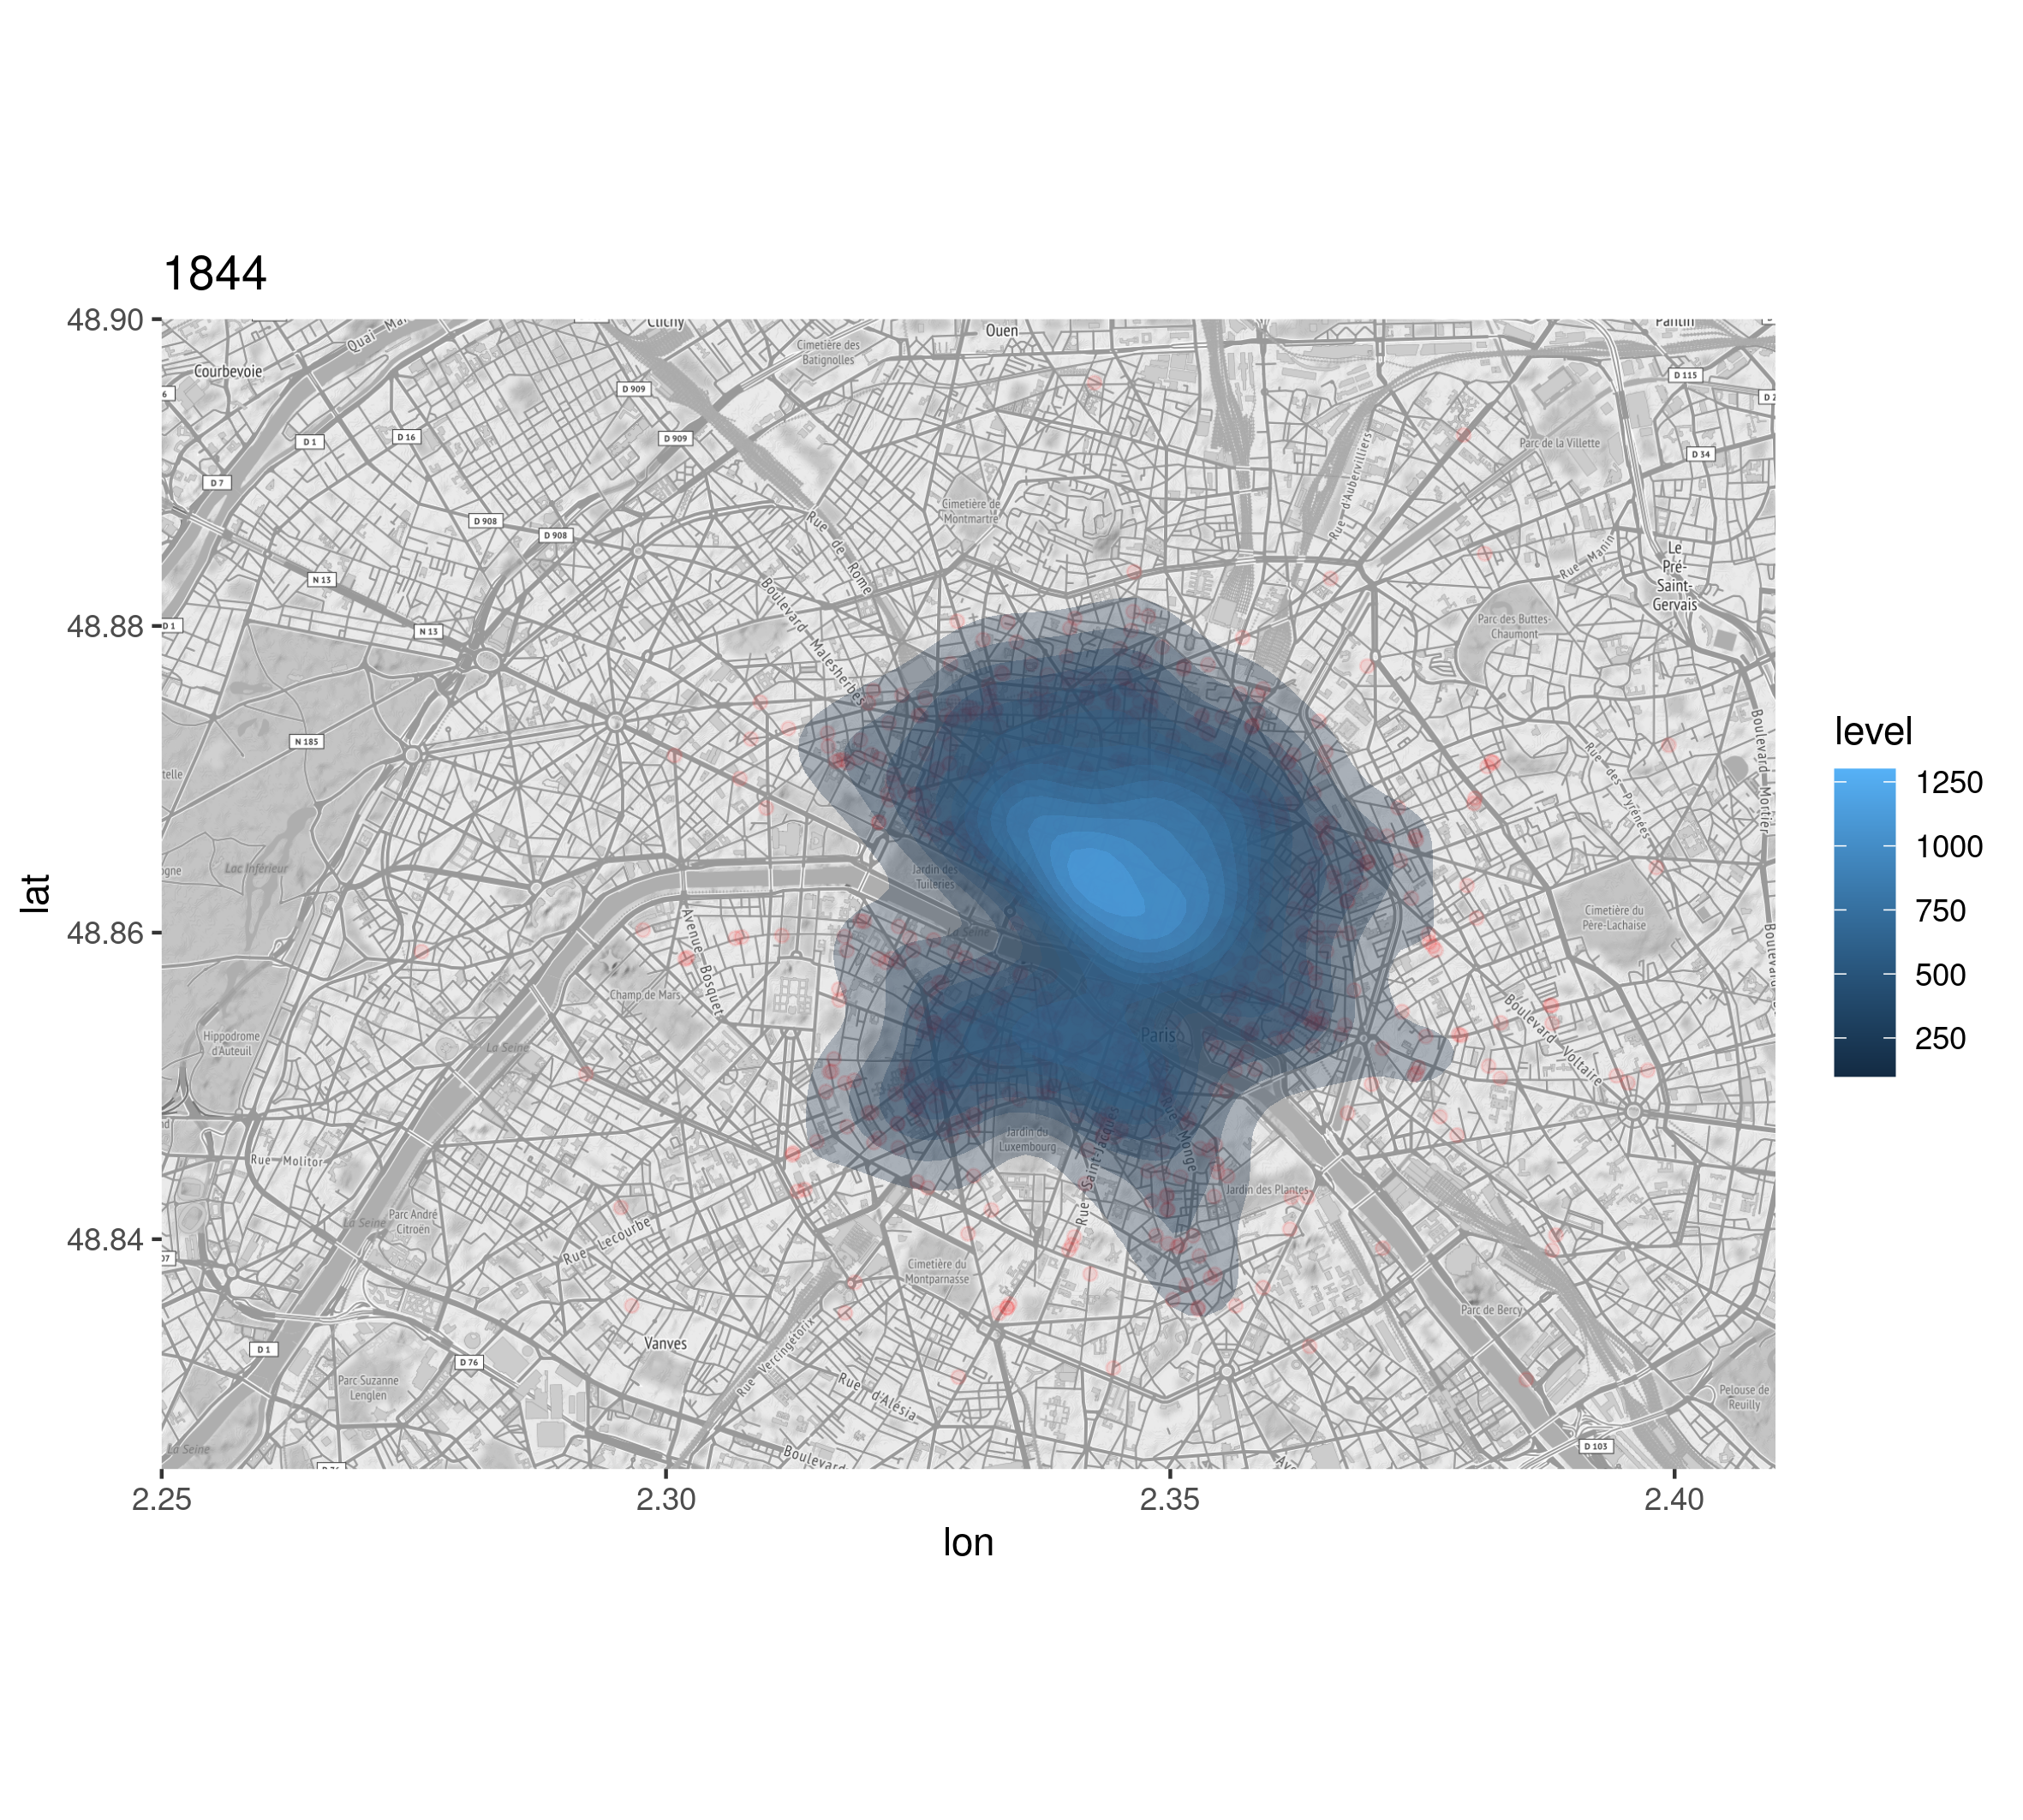
\includegraphics[width=0.49\textwidth, trim={0 0 4.5cm 0}]{figures/density-1844-law.png}
	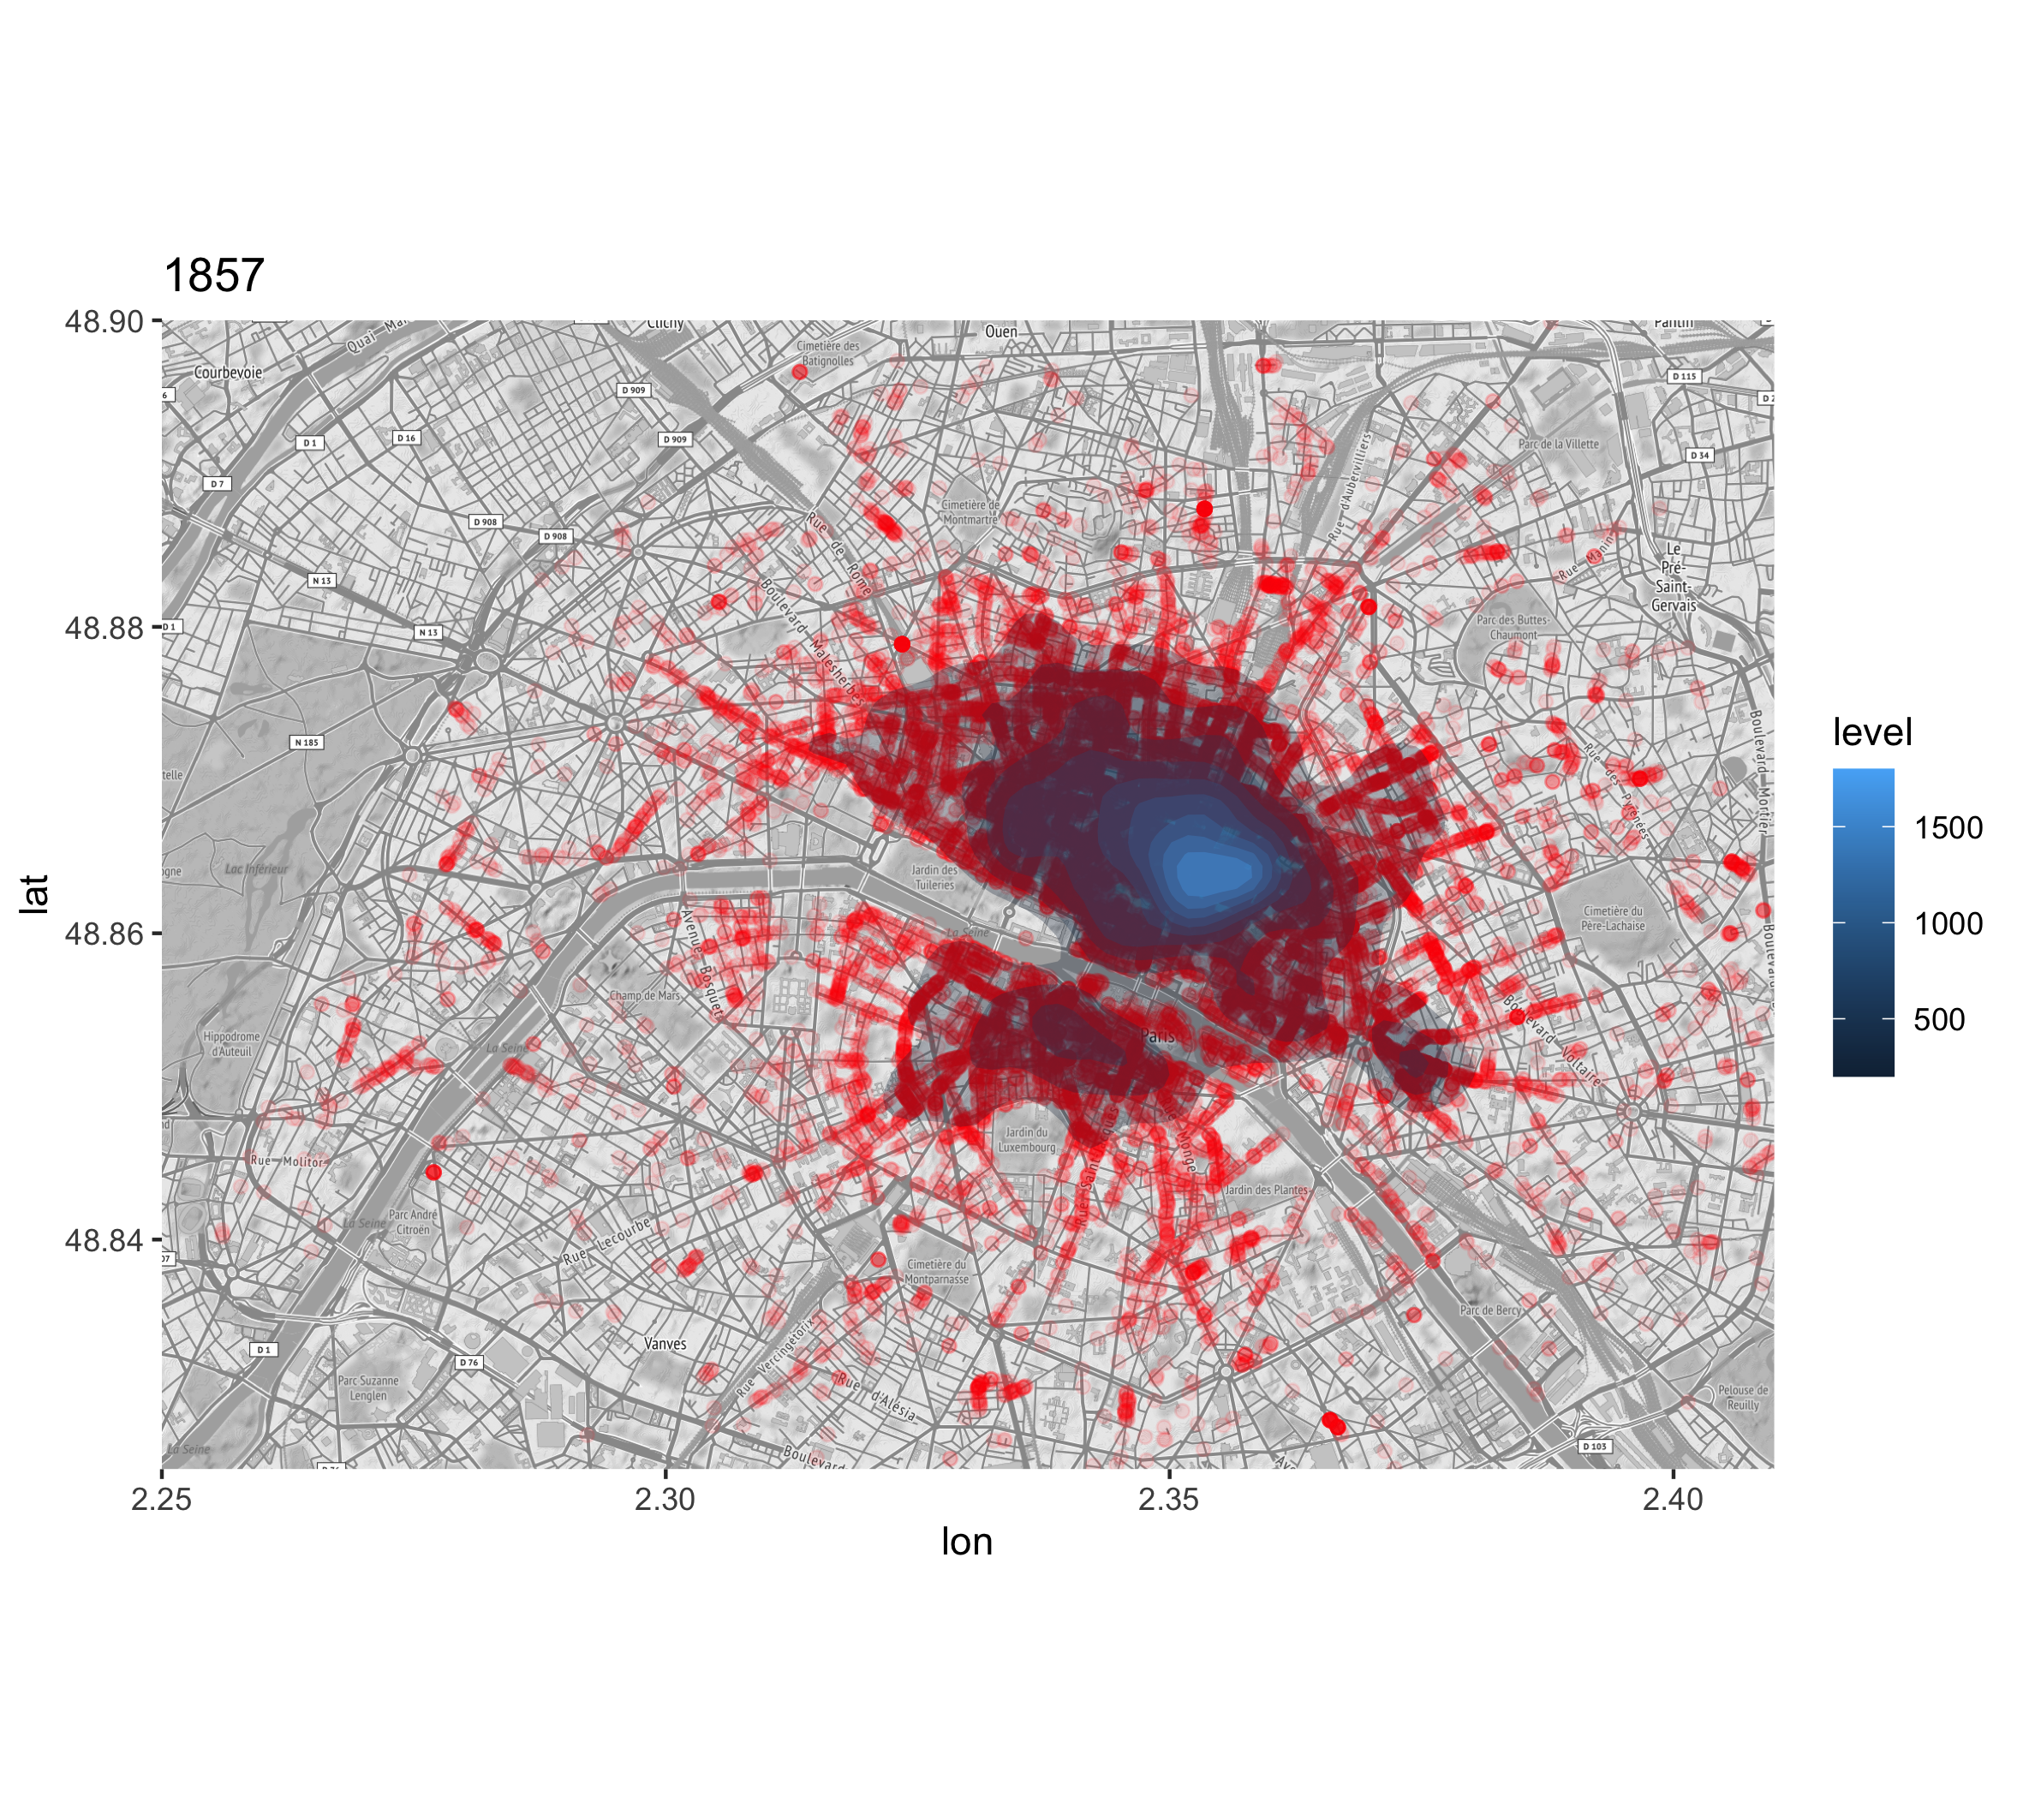
\includegraphics[width=0.49\textwidth, trim={0 0 4.5cm 0}]{figures/density-1857-craftsmanship.png}\hspace{0.1cm}
	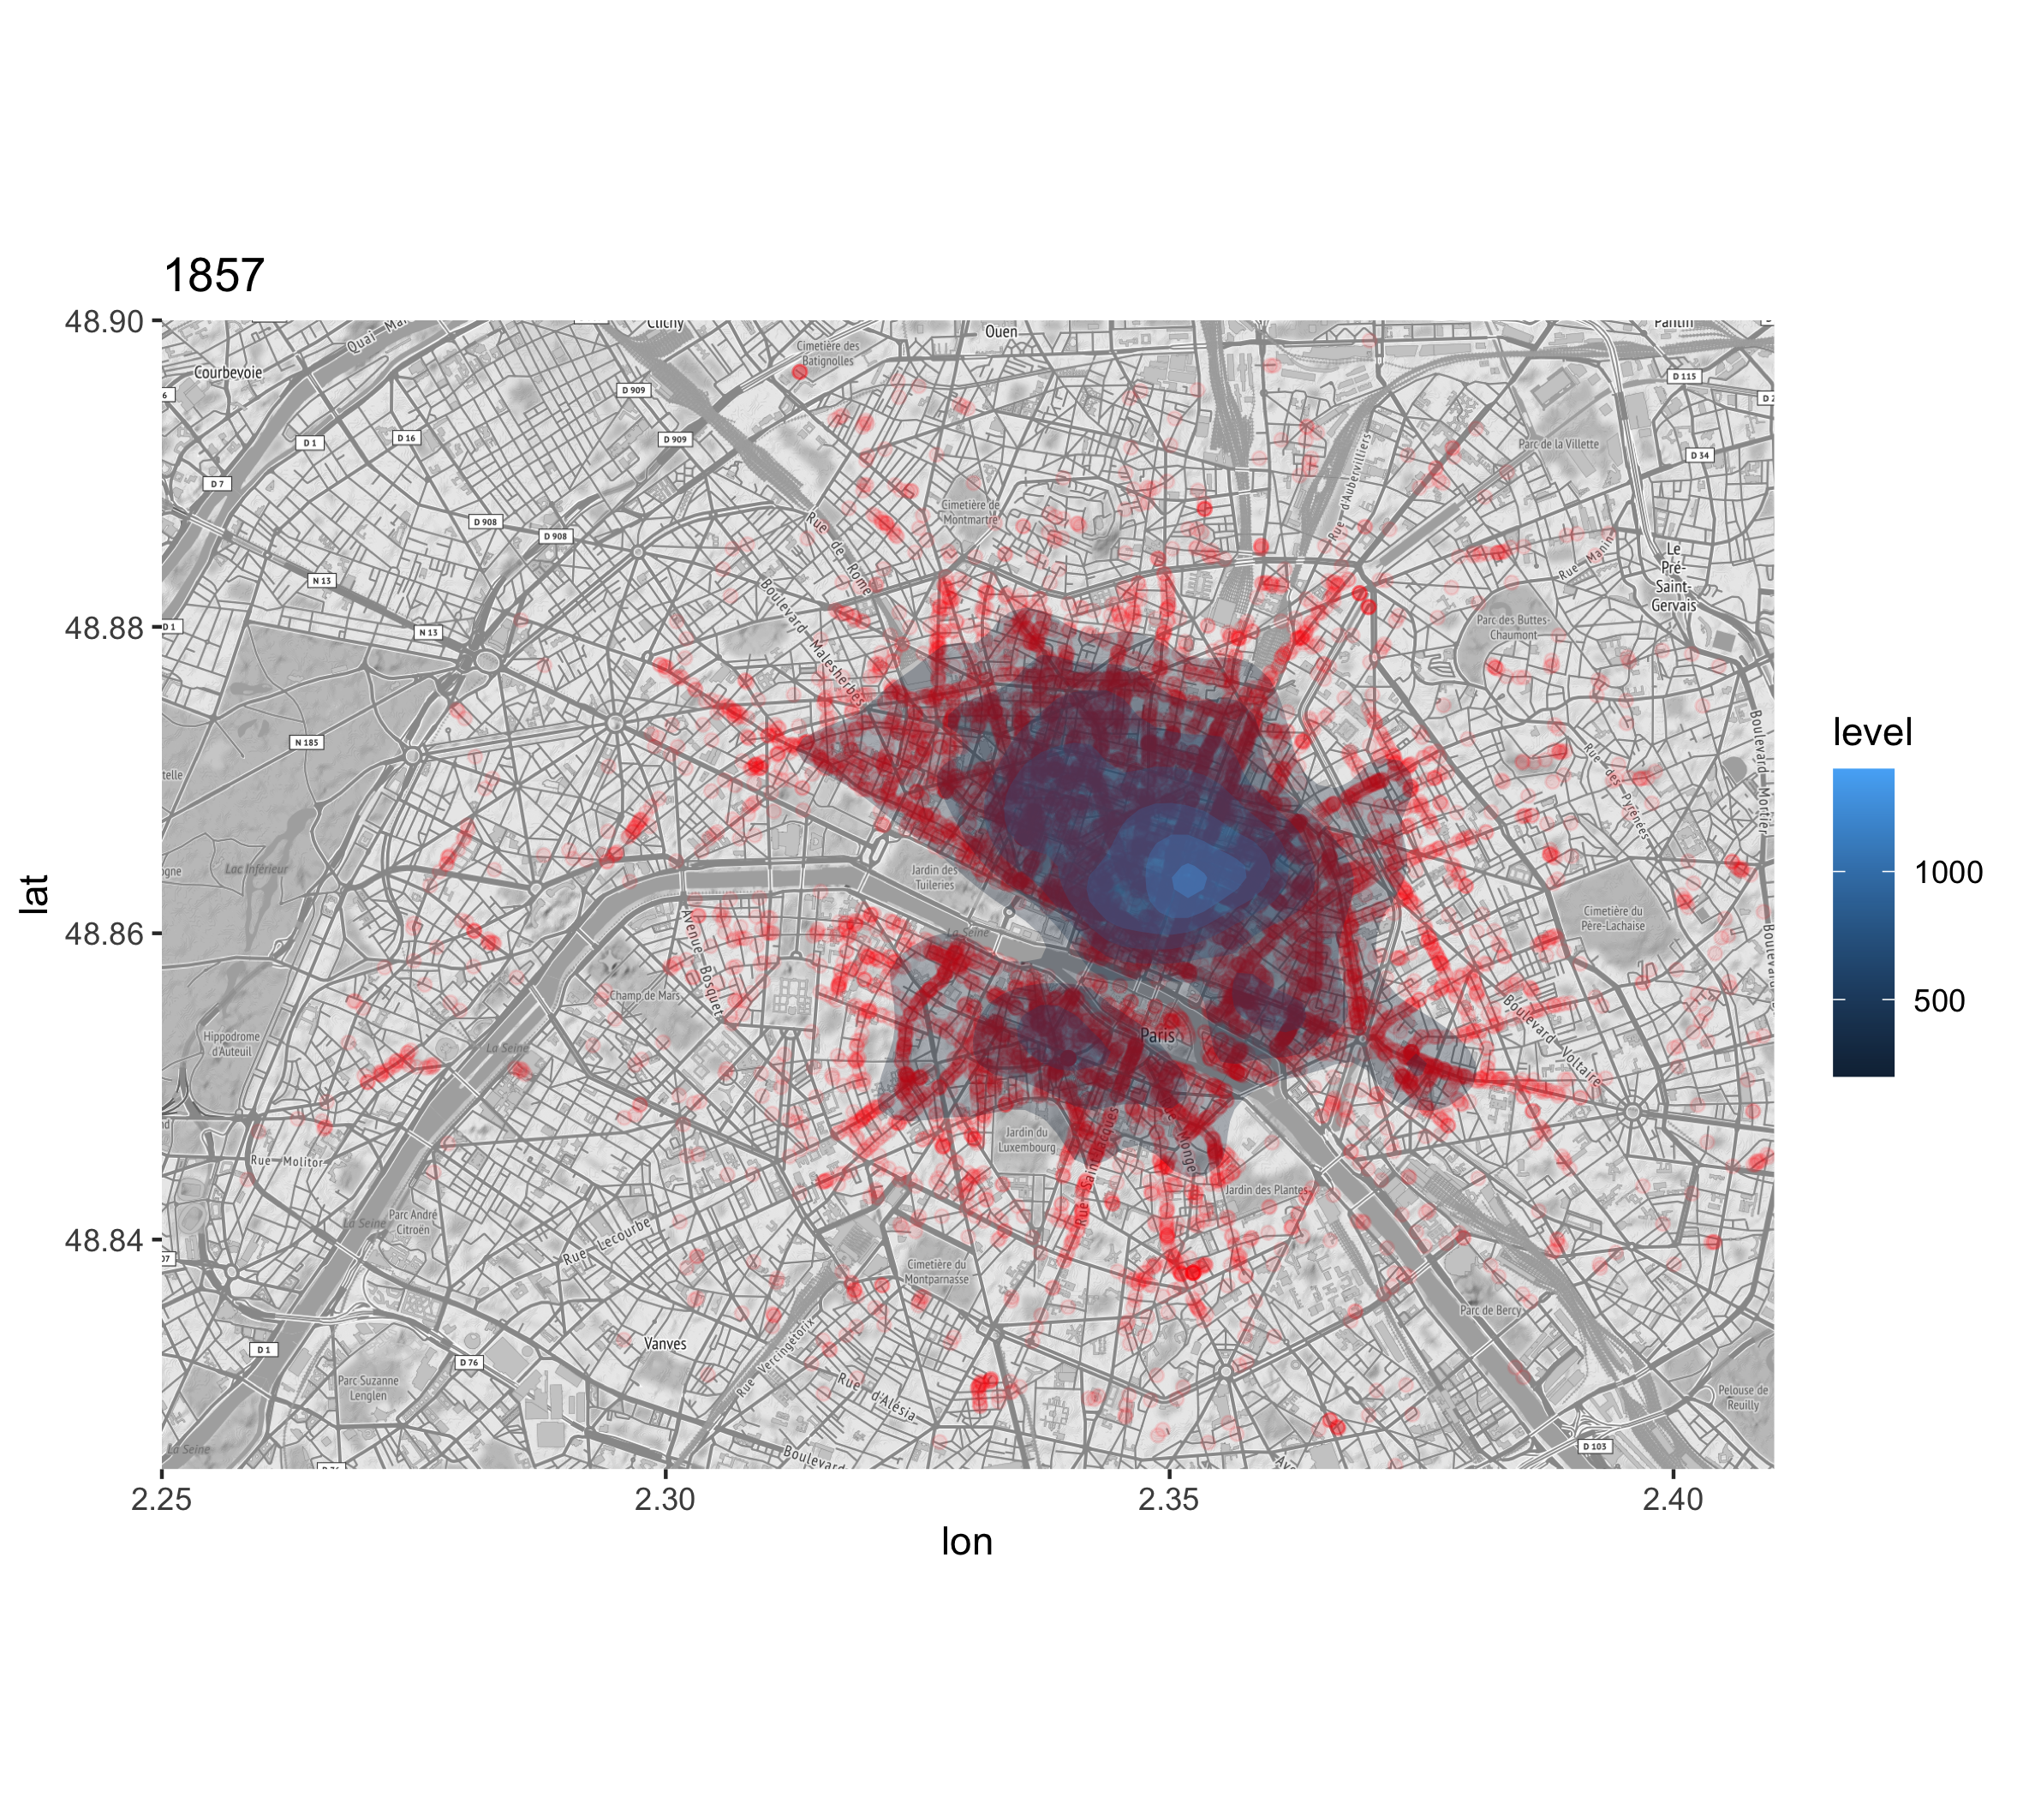
\includegraphics[width=0.49\textwidth, trim={0 0 4.5cm 0}]{figures/density-1857-food.png}
\end{center}

\medskip

Left: craftsmanship; Right: food.


}






\sframe{Defining co-evolution}{


% To study co-evolutionary dynamics, we use the defini- tion and characterisation method proposed by [10], which is based on weak Granger causality: two urban attributes will be co-evolving if they statistically exhibit a circualar causal relationship in this context.
% -> diagram soutenance? -> slides AG soduco

%[10] Juste Raimbault. Characterising and modeling the co- evolution of transportation networks and territories. arXiv preprint arXiv:2110.15950, 2021.



%\justify
 
  \textbf{Objects: } Cities and territories (\textit{Evolutionary Urban Theory} \cite{pumain2018evolutionary}) co-evolving with transport networks (\textit{Territorial Theory of Networks} \cite{dupuy1987vers})
 
 \medskip


\textbf{Processes: }

\textit{A multi-level definition of co-evolution:} 
\begin{enumerate}
	\item \textcolor{blue}{agents level}
	\item \textcolor{green}{agent populations level (niches)}
	\item \textcolor{red}{global system level}
\end{enumerate}  


\medskip


\textbf{Corresponding approaches: }

\begin{enumerate}
	\item \textcolor{blue}{Empirical approach (microscopic level)}
	\item \textcolor{green}{Morphogenesis approach (niche level)}
	\item \textcolor{red}{Evolutionary theory approach (global level)}
\end{enumerate}

\medskip

\tiny

Raimbault, J. (2019). Modeling interactions between transportation networks and territories: a co-evolution approach. arXiv preprint arXiv:1902.04802.
 
 \nocite{raimbault2019modeling}
 
}



\sframe{Method to characterise co-evolution}{

\begin{center}
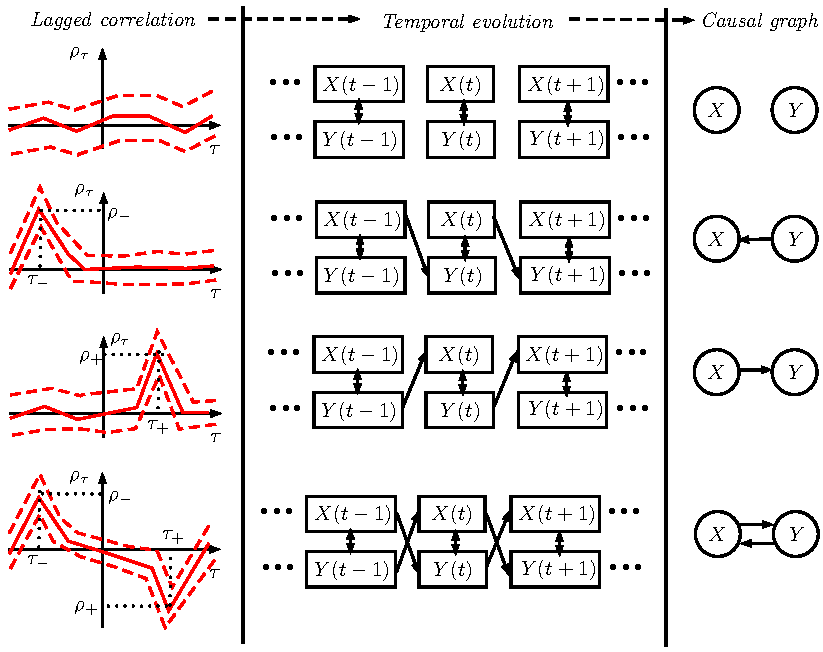
\includegraphics[width=0.8\linewidth]{figures/causality_twovars.pdf}
\end{center}

\tiny

Raimbault, J. (2017). Identification de causalités dans des données spatio-temporelles. In Spatial Analysis and GEOmatics 2017.

\nocite{raimbault2017identification}

}





\sframe{Application to this dataset}{

% Aggregating spatially on raster cells (10x10 grid for the whole Paris), we thus com- pute lagged correlations between the variations of activity counts between successive dates for each cell, for each pair of activity. 

$\rightarrow$ Activity counts $N_{a,r}$ within raster cells: 10x10 grid to split the covered area into zones.

\bigskip

$\rightarrow$ Variation of activity counts in time $\Delta N_{a,r} (t) = N_{a,r}(t+\Delta t) - N_{a,r}(t)$

\bigskip

$\rightarrow$ Lagged correlations in time between activities

\[
\rho_{a_1,a_2}(\tau) = \rho \left[\Delta N_{a_1,r} (t), \Delta N_{a_2,r} (t - \tau) \right]
\]

\bigskip

%$\rightarrow$ On the sample dataset, $\tau = 1$ (3 exploitable dates)


}


\sframe{Results: lagged correlations}{

%We find several significant correlations (using Fisher confidence intervals), mostly negative for lagged cor- relations. This corresponds to a dynamic of sustitution of activities, with clusters rapidly replaced. Food and health are positively correlated and in co-evolution, while the other significantly co-evolving couple of activities is health and art but in a negative manner: in some districts medical pro- fessions replace artists and the contrary in others.


% estimate correlations on time windows - with optim of window size?
% y-by-y diff, corrs / granger caus tests on moving window? OR smooth first (moving window), then tests? bof from thematic viewpoint - variations are fast for such economic activities?


\centering

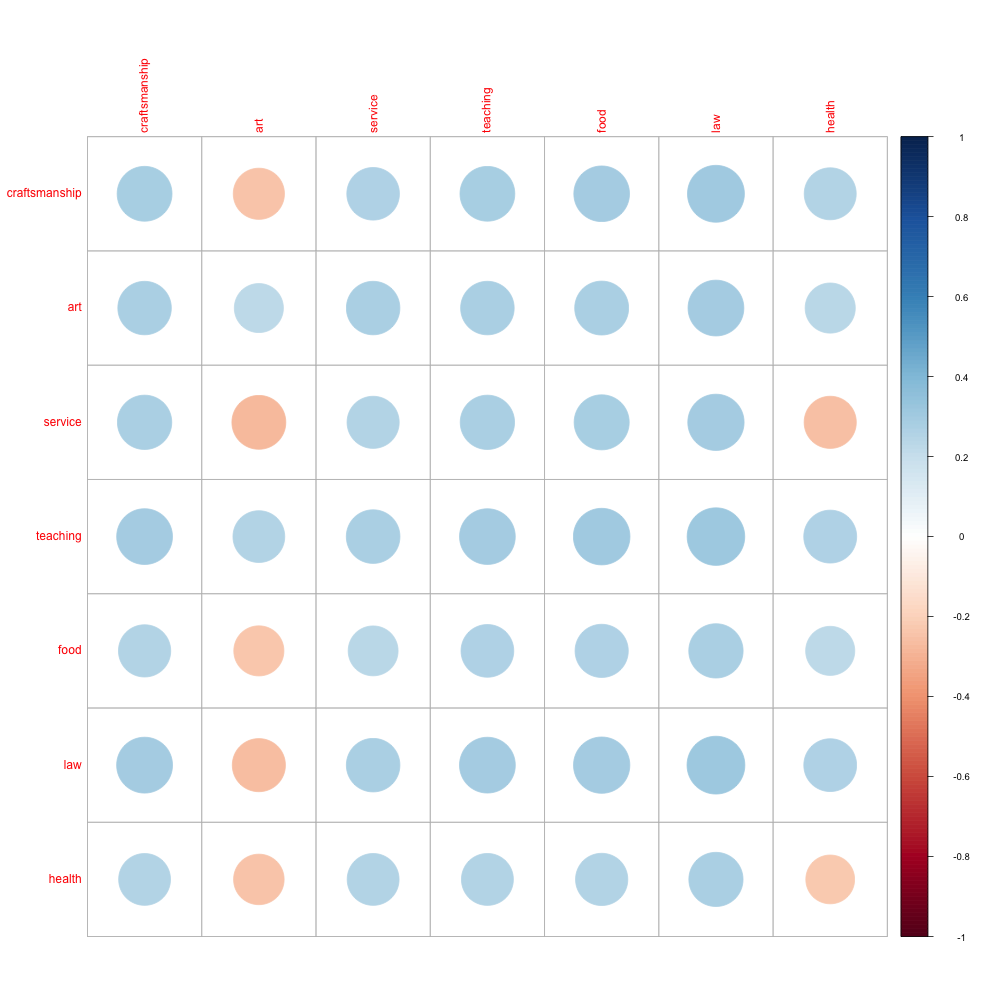
\includegraphics[height=0.8\textheight]{figures/laggedcorrs.png}

\medskip

\textit{Optimal lagged correlations between variations of activity counts}

}

\sframe{Results}{

\centering

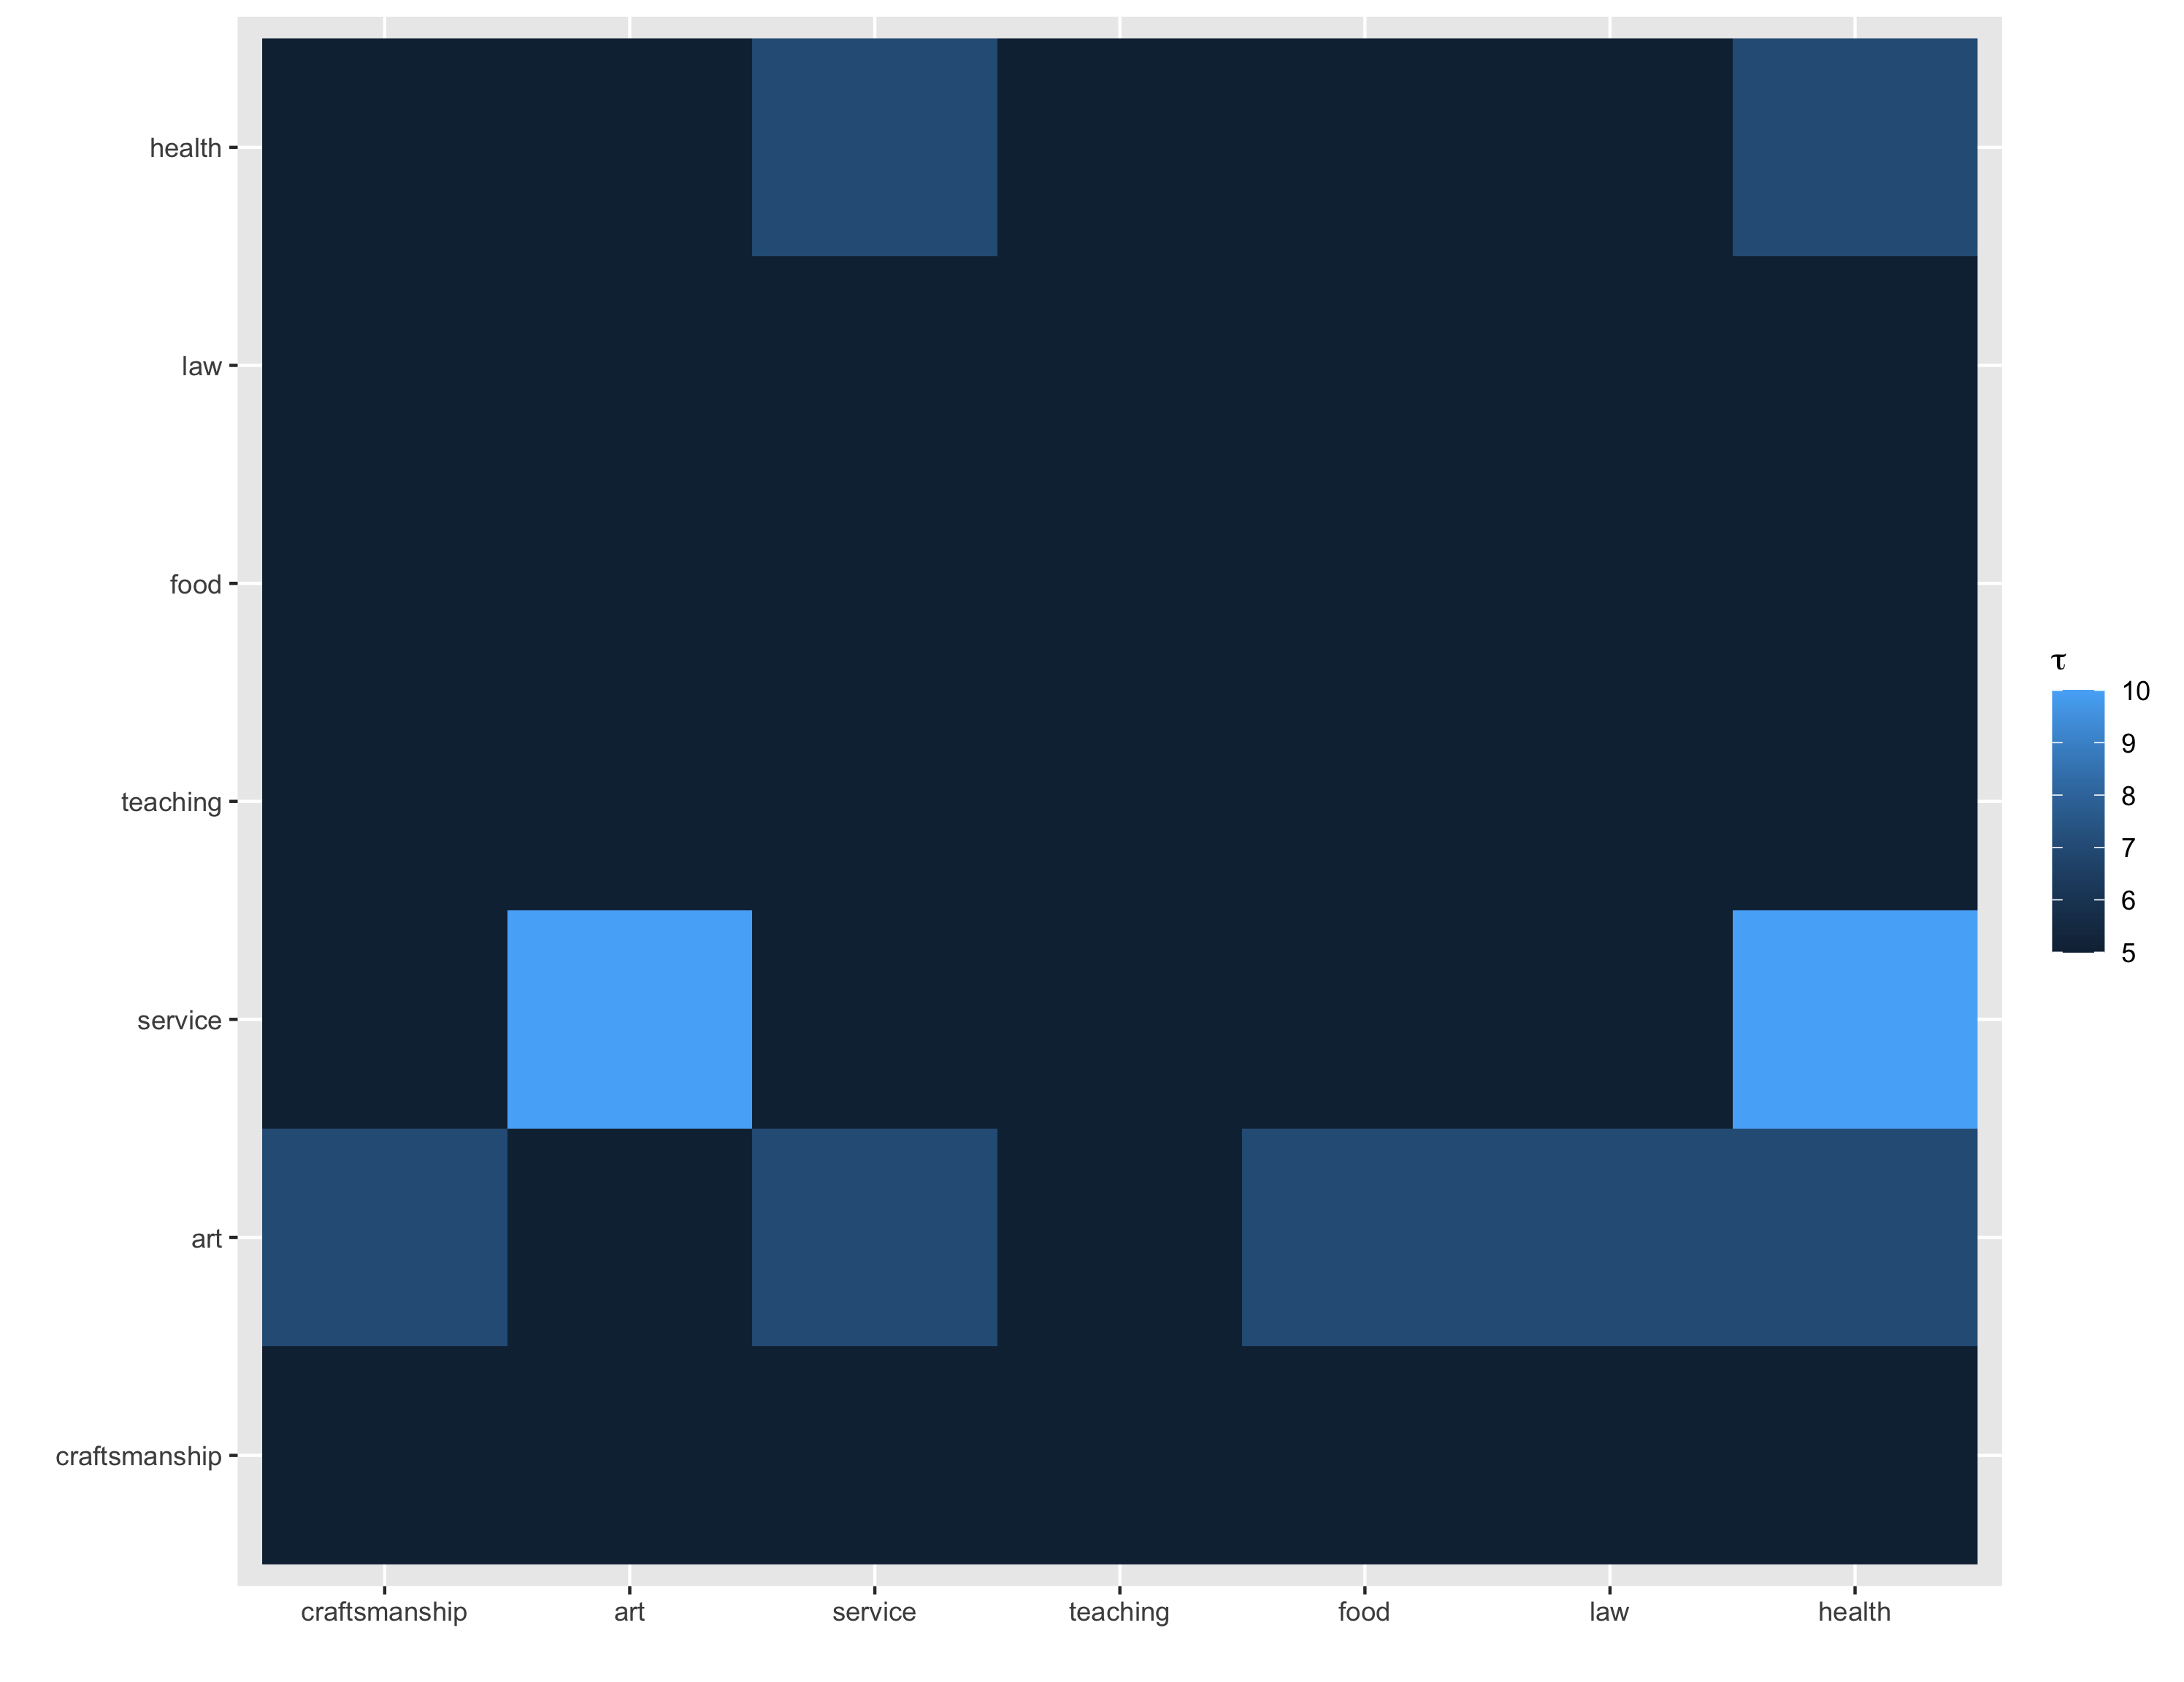
\includegraphics[height=0.8\textheight]{figures/taus.png}

\medskip

\textit{Corresponding delays}


}

%\sframe{Simultaneous correlations}{
%  We also consider simultaneous correlations, and find for example that food and craftsmanship have joint dynamics in the last time interval, but not during the first considered. 

%\centering

%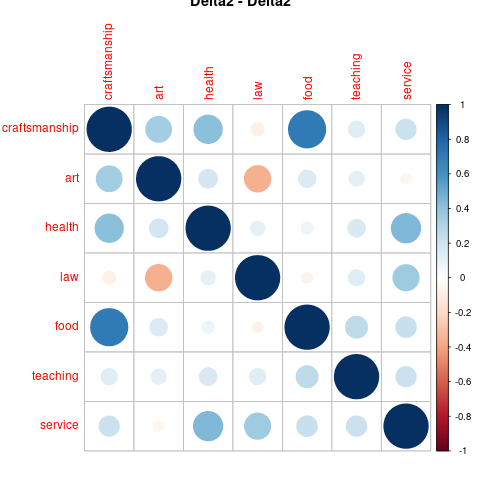
\includegraphics[height=0.9\textheight]{figures/laggedcorrs-22.png}
%}

\section{Discussion}

\sframe{Discussion}{



$\rightarrow$ Micro insights into historical intra-urban economic processes.

\medskip

$\rightarrow$ Existence of a co-evolution between some activities (circular causality in location dynamics).

\medskip

$\rightarrow$ In discussion with historians in the project: capture qualitative knowledge (e.g. ``\textit{fabrique urbaine}'')?


\bigskip

\textbf{Current and future work:}



\medskip

$\rightarrow$ Sensitivity analysis to classification, meta-parameters; null model with random activities.

\medskip

$\rightarrow$ Endogenous spatial neighbourhoods to estimate correlations, using a GWR-like approach \cite{brunsdon1998geographically}; temporal moving-window.
%(// original method) + SENSITIVITY ANALYSIS 

\medskip

$\rightarrow$ Benchmark of methods to measure co-evolution (instrumental variables, causal machine learning, transfer entropy).
% add JR 30/03/2023: TE


}




\sframe{Conclusion}{

$\rightarrow$ Geo-historical data is new data; quantification of past intra-urban processes; many consistence and processing issues.

\medskip

$\rightarrow$ Opening for interdisciplinary discussions and collaborations: actual new knowledge and its validation depends on disciplines.


\bigskip
\bigskip
\bigskip

%\textbf{Soduco website and repository:}
%\url{https://soduco.github.io/}
%\url{https://github.com/soduco}
%\bigskip

\textbf{Models and results open at}



\url{https://github.com/JusteRaimbault/HistoricalData}

}









%%%%%%%%%%%%%%%%%%%%%
\begin{frame}[allowframebreaks]
\frametitle{References}
\bibliographystyle{apalike}
\bibliography{biblio}
\end{frame}
%%%%%%%%%%%%%%%%%%%%%%%%%%%%





\end{document}













